\documentclass{book}
\usepackage{commeunjeustyle}
\begin{document}


\chapter*{Déterminant}
\begin{Texte}%label=introduction_chapter
Pour l'introduire, le déterminant est un nombre que l'on associe à $n$ vecteurs $(\vec{v_1},\ldots,\vec{v_n})$ de $\R^n$.\\
Il correspond au volume du parallélépipède engendré par ces $n$ vecteurs. Le déterminant d'une matrice  est le volume des ses vecteurs colonnes. Le déterminant permet de savoir
si une matrice est inversible ou pas, et de façon plus générale,
détermine l'unicité de la solution d'un système linéaire.
\end{Texte}
\begin{Exemple}[Tailles d'un père et d'un fils] %label=introduction
La somme des tailles d'un fils et du père est de 2,5 mètres. La différence de tailles  est de 0.5 mètres.
Quel est la taille du fils et du père ? \\
Soit la variable $x$ représentant la taille du fils et la variable $y$ représentant la taille du père.\\
Le couple $(x,y)$ vérifie le système suivant  :
$$(S)\quad \begin{cases}
x+y&=2,5\\
-x+y&=0,5
\end{cases}
$$
Avant de déterminer explicitement la solution, un mathématicien se pose des questions sur la structure des solutions du problème. Comme vu au chapitre les espaces vectoriels, le système $(S)$ est équivalent à :
$$	
%\begin{pmatrix}
% 1  & 1  \\ 
% -1 &1   \\
%\end{pmatrix}\times\begin{pmatrix}
%  {\color{red}x}   \\
%  {\color{green}y} \\
%\end{pmatrix}=\begin{pmatrix}
% {\color{blue}2,5}   \\
% {\color{blue}0,5}  \\
%\end{pmatrix}
%\Leftrightarrow
	 {\color{red}x}\begin{pmatrix}
 1    \\
 -1   \\
\end{pmatrix}+{\color{green}y}\begin{pmatrix}
  1   \\
  1  \\
\end{pmatrix}=\begin{pmatrix}
 {\color{blue}2,5}   \\
 {\color{blue}0,5}  \\
\end{pmatrix}$$
En d'autres terme, on cherche les combinaisons linéaires des $(\begin{pmatrix}
 1    \\
 -1   \\
\end{pmatrix},\begin{pmatrix}
 1   \\
  1  \\
\end{pmatrix})$ égales au vecteur $\begin{pmatrix}
 {\color{blue}2,5}   \\
 {\color{blue}0,5}  \\
\end{pmatrix}$

\begin{center}
\begin{tikzpicture}[general,scale=1.5]
\draw [quadrillage] (-0.1,-1.1) grid (3,1.1);
\node[below left,,color=black!30] (0,0) {$O$};
\draw[->,color=black!30] (0,0) -- (1,0) node[below] {$\vec{e_1}$};
\draw[->,color=black!30] (0,0) -- (0,1) node[left] {$\vec{e_2}$};
\draw [->, epais] (0,0) -- (1,-1)node[right]{$\begin{pmatrix}
 1    \\
 -1   \\
\end{pmatrix}$};
\draw [->, epais] (0,0) -- (1,1)node[right]{$\begin{pmatrix}
 1    \\
 1   \\
\end{pmatrix}$};
\draw [->, epais] (0,0) -- (2.5,0.5)node[right]{$\begin{pmatrix}
 {\color{blue}2,5}   \\
 {\color{blue}0,5}  \\
\end{pmatrix}$};
\draw [->, epais] (0,0) -- (2.3,-0.5)node[right]{$ {\color{red}x}\begin{pmatrix}
 1    \\
 -1   \\
\end{pmatrix}+{\color{green}y}\begin{pmatrix}
  1   \\
  1  \\
\end{pmatrix}$};
\end{tikzpicture}
\end{center}
De deux choses l'une,
\begin{itemize}
\item si la famille est une base, alors il existe une unique solution,
\item si la famille n'est pas une base, alors soit il n'existe pas de solution ou une infinité.   
\end{itemize}
En dimension 2,  si les deux vecteurs  ne sont pas colinéaires alors ils forment une base et on a donc existence et unicité de la solution.  Dans notre exemple,  comme les deux vecteurs  $\begin{pmatrix}
 1    \\
 -1   \\
\end{pmatrix}$ et $\begin{pmatrix}
 1   \\
  1  \\
\end{pmatrix}$ ne sont pas colinéaires, il y a existence et  unicité de la  solution.\\
L'idée du déterminant est d'avoir un outil permettant de répondre à cette question : est-ce qu'une famille de $n$ vecteurs est une base  en dimension $n$ ?\\
Dans le plan, le déterminant calcule l'aire orientée du parallélogramme défini par deux vecteurs, $\Vect{u}=\begin{pmatrix}
a\\c
\end{pmatrix}$ et $\Vect{v}=\begin{pmatrix}
b\\d
\end{pmatrix}$  
\begin{center}
\begin{tikzpicture}[scale=1.3,>=latex]
\filldraw[colorprop!20,draw=colorprop] (0,0) -- (2.2,0.3) -- (2.6,1.5) -- (0.4,1.2) -- cycle;
\draw[->,colorprop,thick] (0,0) -- (2.2,0.3) node[right] {$\vec{u}$};
\draw[->,colorprop,thick] (0,0) -- (0.4,1.2) node[above] {$\vec{v}$};
\node[below left,color=black!30] (0,0) {$O$};
\draw[->,color=black!30] (0,0) -- (0.5,0) node[below] {$\vec{e_1}$};
\draw[->,color=black!30] (0,0) -- (0,0.5) node[left] {$\vec{e_2}$};
\end{tikzpicture}
\end{center}
Avec des arguments géométriques, on peut démontrer que l'aire orientée du parallélogramme est donnée par :  
$$
\Fonction{\det}{\R^2\times\R^2}{\R}{\begin{pmatrix}
a\\c
\end{pmatrix},\begin{pmatrix}
b\\d
\end{pmatrix}}{\begin{vmatrix}
a & b \\
c & d
\end{vmatrix}=a d-c d}.
$$
Si les deux vecteurs sont colinéaires, alors l'aire est égale à 0 car la parallélogramme est aplati  sinon l'aire est différente de zéro. C'est-à-dire, la famille $(\Vect{u},\Vect{v})$ est une base si et seulement si le déterminent est différent de zéro. \\
Dans l'espace,  le déterminant calcule le volume du parallélépipède : 
\begin{center}
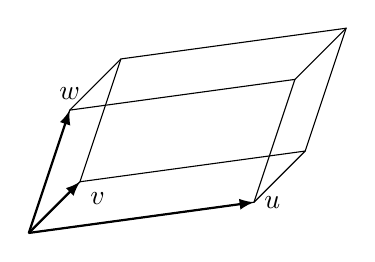
\begin{tikzpicture}[scale=1.3,>=latex]
\draw (0,0) -- (2.2,0.3) -- (2.6,1.5) -- (0.4,1.2) -- cycle;
\draw (0.5,0.5) -- (2.7,0.8) -- (3.1,2.0) -- (0.9,1.7) -- cycle;
\draw (0,0) -- (0.5,0.5);
\draw (2.2,0.3) -- (2.7,0.8);
\draw (2.6,1.5) --  (3.1,2.0);
\draw  (0.4,1.2) --  (0.9,1.7);

\draw[->,thick] (0,0) -- (2.2,0.3) node[right] {$\Vect{u}$};
\draw[->, thick ] (0,0) -- (0.5,0.5) node[below right] {$\Vect{v}$};
\draw[->,thick] (0,0) -- (0.4,1.2) node[above] {$\Vect{w}$};
\end{tikzpicture}
\end{center} 
De nouveau, la famille $(\Vect{u},\Vect{v},\Vect{w})$ est une base si et seulement si le déterminent est différent de zéro.\\
Avec  encore plus de difficulté, on peut démontrer avec des arguments géométriques que le volume  orientée du parallélépipède est donnée par :  
$$
\Fonction{\det}{\R^3\times\R^3\times\R^3}{\R}{\begin{pmatrix}
a\\b\\g
\end{pmatrix},\begin{pmatrix}
b\\e\\h
\end{pmatrix},\begin{pmatrix}
c\\f\\i
\end{pmatrix}}{\begin{vmatrix}
a & b &c \\
d & e &f \\
g & h &i\\
\end{vmatrix}=a(ei-hf)-d(bi-hc)+g(bf-ec) }.
$$
En revanche en  dimension $n$ quelconque, il semble extrêmement difficile de déterminer la formule du volume à base d'arguments géométriques. Une brillante idée est  de déterminer des équations fonctionnelles vérifiées par le déterminant et d'en déduire la formule du volume. \\
En effet,  sur le plan, on remarque que l'aire est :
\begin{enumerate}
\item \impo{Normalisée} : l'aire du carré unité est 1, $\det(\Vect{e_1},\Vect{e_2})=1$
\item \impo{2-linéaire} : linéaire par rapport à chaque une de ces deux variables.
\begin{center}
Pour la linéarité à gauche :\\
\begin{tikzpicture}[scale=1.3,>=latex]
\filldraw[colorprop!20,draw=colorprop] (0,0) -- (2.2,0.3) -- (2.6,1.5) -- (0.4,1.2) -- cycle;
\filldraw[colordef!20,draw=colordef, opacity=0.2] (0,0) -- (1.1,0.15) -- (1.5,1.35) -- (0.4,1.2) -- cycle;
\draw[->,colorprop,thick] (0,0) -- (2.2,0.3) node[below] {$\lambda\vec{u}$};
\draw[->,colordef,thick] (0,0) -- (1.1,0.15) node[below] {$\vec{u}$};

\draw[->,colorprop,thick] (0,0) -- (0.4,1.2) node[above] {$\vec{v}$};

\node[below left,color=black!30] (0,0) {$O$};
\draw[->,color=black!30] (0,0) -- (0.5,0) node[below] {$\vec{e_1}$};
\draw[->,color=black!30] (0,0) -- (0,0.5) node[left] {$\vec{e_2}$};
\end{tikzpicture}\\
${\color{colorprop}\det(\lambda\Vect{u},\Vect{v})}=\lambda{\color{colordef}\det(\Vect{u},\Vect{v})}$\\
\begin{tikzpicture}[scale=1.3,>=latex]
\filldraw[colorprop!50,draw=colorprop, opacity=0.2] (0,0) -- (1.1,0.15) -- (1.5,1.35) -- (0.4,1.2) -- cycle;
\filldraw[colordef!50,draw=colordef, opacity=0.2] (1.1,0.15) -- (2.4,0.7) -- (2.8,1.9) -- (1.5,1.35) -- cycle;
\filldraw[green!50,draw=green, opacity=0.2] (0,0) -- (2.4,0.7) -- (2.8,1.9) -- (0.4,1.2) -- cycle;
\draw[->,colorprop,thick] (0,0)     -- (1.1,0.15) node[below] {$\vec{u}$};
\draw[->,colordef,thick] (1.1,0.15) -- (2.4,0.7) node[below] {$\vec{v}$};
\draw[->,green,thick] (0,0) -- (2.4,0.7) node[right] {$\vec{u}+\vec{v}$};
\draw[->,colorprop,thick] (0,0) -- (0.4,1.2) node[above] {$\vec{w}$};
\draw[->,colordef,thick] (1.1,0.15) -- (1.5,1.35) node[above] {$\vec{w}$};
\node[below left,color=black!30] (0,0) {$O$};
\draw[->,color=black!30] (0,0) -- (0.5,0) node[below] {$\vec{e_1}$};
\draw[->,color=black!30] (0,0) -- (0,0.5) node[left] {$\vec{e_2}$};
\end{tikzpicture}\\
${\color{colorprop}\det(\Vect{u},\Vect{w})}+{\color{colordef}\det(\Vect{v},\Vect{w})}={\color{green}\det(\Vect{u}+\Vect{v},\Vect{w})}$
\end{center}
\item \impo{Alternée} : comme l'aire d'un parallélogramme aplati est 0, si $\Vect{u}=\Vect{v}$ alors $\det(\Vect{u},\Vect{v})=0$ 
\end{enumerate}
Dans l'espace, le volume est :
\begin{enumerate}
\item \impo{Normalisé} : le volume du cube unité est 1, $\det(\Vect{e_1},\Vect{e_2},\Vect{e_3})=1$
\item \impo{3-linéaire} : linéaire par rapport à chaque une de ces trois variables
\item \impo{Alternée} : le volume d'un parallélépipèdes aplati est 0, si $\Vect{u}=\Vect{v}$ ou $\Vect{u}=\Vect{w}$ ou $\Vect{v}=\Vect{w}$ alors $\det(\Vect{u},\Vect{v},\Vect{w})=0$ .
\end{enumerate}
Ainsi en dimension $n$, le volume devrait être 
\begin{enumerate}
\item \impo{Normalisé} : le volume du cube unité est 1, $\det(\Vect{e_1},\dots,\Vect{e_n})=1$
\item \impo{$n$-linéaire} : linéaire par rapport à chaque une de ces $n$ variables
\item \impo{Alternée} : le volume d'un parallélépipèdes aplati est 0,  si $\Vect{u_i}=\Vect{u_j}$ avec $i\neq j$,  alors $\det(\Vect{u_1},\dots,\Vect{u_n})=0$.
\end{enumerate}
Le théorème important est qu'il existe une unique application vérifiant ces trois propriétés. De plus, ce théorème fournit une formule pour le calculer.\\
Dans la suite, les vecteurs sont rangés sous forme d'une matrice, par exemple $$\det(\vec{u}=\begin{pmatrix}
a  \\
c \\
\end{pmatrix} ,\vec{v}=\begin{pmatrix}
b  \\
d \\
\end{pmatrix})=\det(\begin{pmatrix}
a & b \\
c & d
\end{pmatrix}).$$ 
  
\end{Exemple}
\section{Définition}
\begin{Theoreme}[Unicité et existence du déterminant]
Soit $E$ un espace vectoriel de dimension. Soit $\mathcal{B}=(\Vect{e_1},\dots,\Vect{e_n})$ une base de $E$.\\
Il existe une unique application $\det: E^n\to\K$ vérifiant les propriétés suivantes:
\begin{enumerate}
\item \propri{Normalisé} : $\det(\Vect{e_1},\dots,\Vect{e_n}) = 1$
\item \propri{$n$-linéaire} : linéaire par rapport à chaque une de ces $n$ variables
\item
  \propri{Alternée} : $\det(\Vect{e_1},\dots,\Vect{e_n}) = 0$ si $\Vect{e_i}=\Vect{e_j}$ pour $i\neq j$.
\end{enumerate}
\end{Theoreme}


\begin{Theoreme}[Unicité et existence du déterminant]
Soit $n\in  \N^*$.
Il existe une unique application $\det: \MnK\to\K$ vérifiant les propriétés suivantes:
\begin{enumerate}
\item \defi{Normalisé} : $\det(\mathrm{I}_n) = 1$;
\item
  \defi{Alternée} : $\det(A) = 0$ si deux colonnes de $A$ sont égales;
\item \defi{$n$-linéaire} :
  Si on fixe $n-1$ colonnes de $A$, l'application qui à la dernière colonne associe $\det(A)$ est linéaire.
  $$\det(C_1 \dots  \lambda C_i+ \mu C'_i  \dots C_n) = \lambda \det(C_1 \dots C_i \dots C_n) + \mu  \det(C_1 \dots C'_i \dots C_n).$$
\end{enumerate}
\end{Theoreme}
\begin{Demonstration}
% Soit $\vec{x_1},\dots,\vec{x_n}\in E$; les composantes de $\vc x_j$ dans
%$\mcal{B}$ sont notées $a_{i,j}$ et pour $f\in\Lambda_n^*(E)$, on écrit
%\begin{align*}
%f\nuple{\vc x}
% &=f\Bigl(\sum_{i_1=1}^n a_{i_1,1}\vc e_{i_1},\vc x_2,\dots,\vc x_n\Bigr)   \\
% &=\sum_{i_1=1}^n a_{i_1,1} f(\vc e_{i_1},\vc x_2,\dots,\vc x_n)
%  \quad\text{ linéarité de $f$ par rapport à $\vc x_1$}       \\
% &=\sum_{1\leq i_1,\dots,i_n\leq n}a_{i_1,1}\dots a_{i_n,n}
%  f(\vc e_{i_1},\dots,\vc e_{i_n})
%  \quad\text{$n$-linéarité de $f$}
%\end{align*}
%Étant donnés $(i_1,\dots,i_n)\in\Intf1n^n$, on pose $s(k)=i_k$
%pour $k\in\Intf1n$. Si $s$ n'est pas injective, deux vecteurs
%$\vc e_{s(k)}$ sont égaux et, puisque que $f$ est alternée,
%$$
%f(\vc e_{i_1},\dots,\vc e_{i_n})=f(\vc e_{s(1)},\dots,\vc e_{s(n)})=0
%$$ 
%Sinon $s$ est bijective et appartient à $\sym$, et
%$$
%f(\vc e_{i_1},\ldots,\vc e_{i_n})=f(\vc e_{s(1)},\ldots,\vc e_{s(n)})=
%\eps(s) f(\vc e_1,\ldots,\vc e_n)
%$$
%Ainsi
%\begin{align*}
%f\nuple{\vc x}
% &=\sum_{1\leq i_1,\dots,i_n\leq n}a_{i_1,1}\dots a_{i_n,n}
%  f(\vc e_{i_1},\dots,\vc e_{i_n})                 \\
% &=\sum_{s\in\sym} a_{s(1),1}\dots a_{s(n),n}
%  f(\vc e_{s(1)},\dots,\vc e_{s(n)})                \\
% &=\Bigl(\sum_{s\in\sym} \eps(s) a_{s(1),1}\dots a_{s(n),n}\Bigr)
%  f(\vc e_1,\dots,\vc e_n)                     \\
% &=\Bigl(\sum_{s\in\sym}\eps(s)\prod_{j=1}^n a_{s(j),j}\Bigr)
%  f(\vc e_1,\dots,\vc e_n)
%\end{align*}
% Posons $i=s(j)$ soit $j=s^{-1}(i)$;
%on obtient $\prod_{j=1}^n a_{s(j),j}=\prod_{i=1}^n
%a_{i,s^{-1}(i)}$; comme l'application $s\to s^{-1}$ est une
%bijection de $\sym$ (c'est même une involution) et
%$\eps(s^{-1})=\eps(s)^{-1}=\eps(s)$, on peut écrire, en effectuant
%le changement d'indice de sommation $\sigma=s^{-1}$
%$$
%\sum_{s\in\sym}\eps(s)\prod_{j=1}^n a_{s(j),j}
%=\sum_{s\in\sym}\eps(s^{-1})\prod_{i=1}^n a_{i,s^{-1}(i)}
%=\sum_{\sigma\in\sym}\eps(\sigma)\prod_{i=1}^n a_{i,\sigma(i)}
%$$
\end{Demonstration}



\begin{Proposition}[Propriétés]
Cette application $\det$ vérifie alors automatiquement les propriétés suivantes:
\begin{enumerate}
\item \defi{antisymétrique } : 
  $$\det(C_1 \dots C_i \dots C_j  \dots C_n) = -\det(C_1 \dots C_j \dots C_i  \dots C_n)\text{ si }i\neq j$$
\item \defi{stable par combinaison linéaire} :
  $$\det(C_1 \dots C_i  \dots C_n) =\det(C_1 \dots C_i+\lambda C_j  \dots C_n)\text{ si }i\neq j$$
\item \defi{homothétie d'une colonne} :
  $$\det(C_1 \dots \lambda C_i  \dots C_n) =\lambda\det(C_1 \dots C_i  \dots C_n)$$
  En particulier,
  $$\det(\lambda A) =\lambda^n\det(A)$$
\item  \defi{stable par transposition} $$\det (A) = \det (\transposee{A})$$
\item  \defi{multiplication} $$\det (AB) = \det (A)\det(B)$$
\item  \defi{inversible}  $\det(A) \neq 0$ si et seulement si $A$ est inversible. Si $A$ est inversible, son inverse est donnée par :
$$ A^{-1}=\frac {1}{\det A} {\transposee{\text{com}A}}$$
où $\transposee{\text{com}A}$ est la transposée de la comatrice de $A$.
\end{enumerate}
Dans toutes les propriétés précédentes, on peut remplacer les opération sur les colonnes par des opération sur les lignes.
\end{Proposition}
\begin{Proposition}[Matrice triangulaire] Le déterminant d'une matrice triangulaire,$\begin{pmatrix}a_{11}&a_{12}&\cdots &\cdots &a_{1n}\\0&a_{22}&&&a_{2n}\\\vdots &\ddots &\ddots &&\vdots \\\vdots &&\ddots &\ddots &\vdots \\0&\cdots &\cdots &0&a_{nn}\\\end{pmatrix}$,  est égale au produit des coefficients de la diagonale, soit $a_{11}\times a_{22} \times\dots\times a_{nn}$.
\end{Proposition}
\begin{Definition}[Déterminant d'un endomorphisme]
Soit $E$ un $\K $-espace vectoriel de dimension finie et $u$ un endomorphisme de $E$.\\
Soit $\mathcal{B}$ une base de $E$ et $M$ la matrice de $u$ dans la base $\mathcal{B}$.\\
La quantité $\det(M)$ ne dépendant pas du choix de la base $\mathcal{B}$, mais seulement de $u$, on l'appelle \defi{déterminant} de l'endomorphisme $u$ et on note $\det(u) = \det(M)$.
\end{Definition}
\begin{Exemple}[Déterminant de Vandermonde]

Soit $a_1,\dots,a_n \in  \K ^n$.
La \defi{matrice de Vandermonde} associée à $(a_1,\dots,a_n)$ est
\[ M = \begin{pmatrix}
    1 &  1 &  1 &  \dots &  1  \\
    a_1 &  a_2 &  a_3 &  \dots &  a_n  \\
    a_1^2 &  a_2^2 &  a_3^2 &  \dots &  a_n^2  \\
    \vdots &  \vdots &  \vdots &   &  \vdots  \\
a_1^{n-1} &  a_2^{n-1} &  a_3^{n-1} &  \dots &  a_n^{n-1}  \end{pmatrix}. \]
Le \defi{déterminant de Vandermonde} $V(a_1,\dots,a_n)$ est le déterminant de la matrice de Vandermonde ci-dessus. On a :
$$V(a_1,\dots,a_n) = \prod_{1\leq i < j\leq n} (a_j - a_i). $$
En particulier,
\begin{itemize}
\item $V(a) = 1$,
\item $V(a,b) = b-a$,
\item $V(a,b,c) = (b-a)(c-a)(c-b)$.
\end{itemize}
La matrice de Vandermonde associée à $(a_1,\dots,a_n)$ est inversible si et seulement si les nombres $(a_1,\dots,a_n)$ sont deux à deux distincts.
\end{Exemple}








\end{document}
